\documentclass[11pt, oneside]{article}   	% use "amsart" instead of "article" for AMSLaTeX format
\usepackage{geometry,graphicx}
\geometry{
  top = 23mm,
  left = 18mm, 
  right = 18mm,
  bottom = 25mm,
}
\renewcommand{\baselinestretch}{1.05}
\newcommand\tab[1][1cm]{\hspace*{#1}}
\newcommand\ftab[1][5cm]{\hspace*{#1}}
\newcommand\ttab[1][2cm]{\hspace*{#1}}
\newcommand\tsp[1][0.2cm]{\hspace*{#1}}
\usepackage[]{algorithm2e}
\geometry{letterpaper}
\usepackage{graphicx}
\usepackage{amssymb}
\usepackage{amsthm}
\usepackage{titlesec}
\titlespacing*{\section}
{0pt}{1.5\baselineskip}{1\baselineskip}
\theoremstyle{definition}
\newtheorem{definition}{Definition}[section]

%\usepackage{parskip}

\graphicspath{ {images/} }

\newtheorem*{theorem}{Theorem}
\newtheorem*{lemma}{Lemma}
%SetFonts

\title{Dijkstra's Algorithm Verification}
\author{Yazhe Feng}
%\date{}							% Activate to display a given date or no date

\begin{document}
\maketitle

\section{Dijkstra's Algorithm}

\subsection{Pseudocode}
Given input graph $g$ and source node $s$ with types:
\\\\
  \tab g : Graph gsize weight\\
  \tab s : Node gsize
\\\\
We denote $(u, v)$ as an edge from node $u$ to $v$, $weight(u, v)$ as the weight of edge $(u, v)$. We define $unexplored$ as the list of unexplored nodes, and $dist$ as the list storing distance from $s$ to each node $n \in g$
\\\\
\tab (initially $unexplored$ contains all nodes in graph $g$)\\
\tab $unexplored : List (Node \tsp gsize)$\\
\tab $unexplored = \{v : v \in g\}$
\\\\
\tab (node value is used to index $dist$, initially distance of all nodes are infinity except 
\\ \tab the source node)\\
\tab $dist : List \tsp weight$ \\
\tab $dist[s] = 0, dist[a] = infinity, \forall a \in g, a \neq s$
\\\\
The Dijkstra's Algorithm runs as follows: 
\\\\
\texttt{
  \tab while (unexplored is not Nil) 
  \tab$\{$ \\
  \tab\tab (At the $k^{th}$ iteration of the while loop)                                          \\
  \tab\tab choose $u \in unexplored$ s.t.$\forall u' \in unexplored, dist[u] \leq dist[u']$     \\
  \tab\tab let $unexplored'$ be the list after removing $u$ from $unexplored$                    \\
  \tab\tab for($\forall v \in g$ s.t.$(u, v) \in g$) $\{$                                 \\  
  \tab\tab\tab (At the $p^{th}$ iteration of this for loop)                                \\
  \tab\tab\tab  if($dist[u] + weight(u, v) < dist[v]$) $\{$                              \\
  \tab\tab\tab\tab  let $dist' = dist$ with $dist'[v] = dist[u] + weight(u, v)$          \\
  \tab\tab\tab $\}$ \\ 
  \tab\tab\tab input the new $dist'$ to the $(p+1)^{th}$ iteration of the for loop \\
  \tab\tab $\}$ \\
  \tab\tab input the new $unexplored'$ and $dist'$ to the $k^{th}$ iteration of the while loop \\
  \tab $\}$
}

\subsection{Assumptions}
\begin{enumerate}
  \item Weight of edges are positive
  \item Distance value can only be zero, infinity, or summation of edge weights
  \item All nodes $n$ and edge $e$ are valid: $n, e \in g$
\end{enumerate}



\section{Definition}
\theoremstyle{definition}
\begin{definition}\textbf{Path}\\
\textit{(We adopt the definition of $path$ presented in the \texttt{Discrete Mathematics with Applications} book by \texttt{SUSANNA S. EPP}.)}
\\\\
A path from node $v$ to $w$ is a finite alternating sequence of adjacent vertices and edges of G, which does not contain any repeated edge or vertex. A path from $v$ to $w$ has the form: 
\begin{center}
 $ve_0v_0e_1v_2....v_{n-1}e_nw$ 
\end{center}
where $e_i$ is an edge in $g$ with endpoints $v_{i-1}, v_i$. We denote the set of paths from $v$ to $w$ as $path(v, w)$.
\end{definition}
\tab
\begin{definition}\textbf{Length of Path} \\
The length of a path $p = ve_0v_0e_1v_2....v_{n-1}e_nw$ is the sum of the weights of all edges in $p$. We write: 
\begin{center}
  $length(p) = \sum weight(e_i), \forall e_i \in p$. 
\end{center} 
\end{definition}
\tab
\begin{definition}\textbf{Shortest Path}\\
Denote $\Delta(s, v)$ as the shortest path from $s$ to $v$, and $\delta(v)$ as the length of $\Delta(s, v)$. $\Delta(s, v)$ must fulfills: 
\begin{center}
$\Delta(s, v) \in path(s, v)$ 
\\
and 
\\
$\forall p' \in path(s, v)$, $\delta(v) = length(\Delta(s, v)) \leq length(p')$
\end{center}
\end{definition}

\section{Proof of Correctness}
\subsection{Proof of Termination}
The inner for loop is guaranteed to terminate as the algorithm goes through each adjacent node exactly once. As the size of list \texttt{unexplored} decreases by one during each iteration of the while loop, the algorithm is guaranteed to terminate. 


\subsection{Proof of Correctness}
Given graph $g$ and source node $s$, $dist$ stores the distance value from $s$ to all nodes in $g$ calculated by the Dijkstra's algorithm, $dist[v]$ gives the corresponding distance value of $v$ from $s$. Denote $explored$ as the list of nodes in $g$ but not in $unexplored$, i.e., $explored$ stored all nodes whose neighbors have been updated by the algorithm, and $dist_{k}[v]$ as the value of $dist[v]$ during the $k^{th}$ iteration of the algorithm. 
\newpage
\begin{lemma}
[1] During the $n^{th}$ iteration of the algorithm for $n \geq 1$, forall node $v \in explored$, we have:
\begin{enumerate}
  \item $\delta(v) \leq \delta(v')$, $\forall v' \in unexplored$.
  \item $dist_n[v] = \delta(v)$
\end{enumerate}
\end{lemma}
\begin{proof}
We will prove this by inducting on the number of iterations. 
\\\\
Let P(n) be: during the $n^{th}$ iteration of the algroithm for $n \geq 1$, forall node $v \in explored$: (1) $\delta(v) \leq \delta(v')$, $\forall v' \in unexplored$; and (2) $dist_n[v] = \delta(v)$. 
\tab\\\\
\textbf{Base Case}: We shall show P(1) holds \\
Based on the algorithm, during the first iteration, the node with minimum distance value is the source node $s$ with $dist_1[s] = 0$. Hence during the first iteration, only $s$ is removed from $unexplored$ and added to $explored$. Since all edge weights are positive, then the shortest distance value from $s$ to $s$ is indeed $0$, hence $dist_1[s] = 0 = \delta(s)$ and $\delta(s) \leq \delta(v')$, $\forall v' \in unexplored$. P(1) holds.
\\\\
\textbf{Inductive Hypothesis}: Suppose P(i) is true for all $1 < i \leq k$. That is, during the $i^{th}$ iteration forall $1 < i \leq k$, forall node $v \in explored$: (1) $\delta(v) \leq \delta(v')$, $\forall v' \in unexplored$; and (2) $dist_i[v] = \delta(v)$. 
\\\\
\textbf{Inductive Step}: We shall show P(k+1) holds.
\\
Suppose $v$ is the node added into $explored$ during the $(k+1)^{th}$ iteration. We need to show (1) $\delta(v) \leq \delta(v')$, $\forall v' \in unexplored$, and (2) $dist_{k+1}[v] = \delta(v)$. 
\begin{enumerate}
\item $\delta(v) \leq \delta(v')$, $\forall v' \in unexplored, v' \neq v$
\\\\
We will prove (1) by contradiction. Suppose there exists $w \in unexplored$, such that $\delta(v) > \delta(w)$. 
\\
Based on the definition of shortest path, $\delta(v) \leq dist_{k+1}[v]$. Since $\delta(v) > \delta(w)$ and $\delta(v) \leq dist_{k+1}[v]$, then we have $\delta(w) < dist_{k+1}[v]$([1]). 
\\
Let $p_w$ be the shortest path from $s$ to $w$, i.e., $\delta(w) = length(p_w)$. Since $w \notin explored$ during the $(k+1)^{th}$ iteration, then there must exists some node along $p_w$ that are not in $explored$. Suppose during the $(k+1)^{th}$ iteration, the first node in $p_w$ that is not in the $explored$ list is $w_2$, and the node right before $w_2$ in the $s$ to $w_2$ subpath is $w_1$, thus $w_1 \in explored$ during the $(k+1)^{th}$ iteration. The image below illustrates this construction: 
\\
\begin{center}
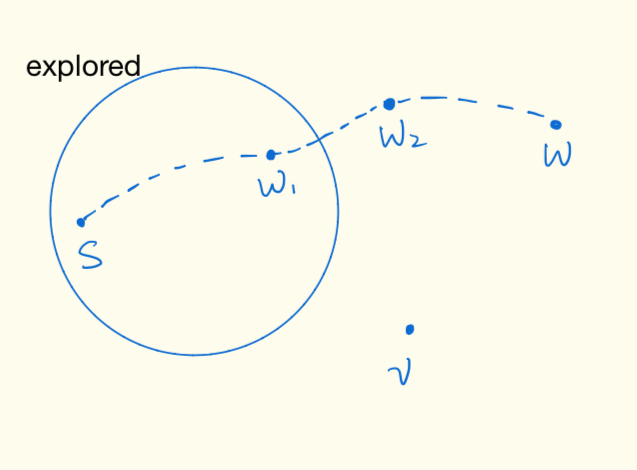
\includegraphics[scale = 0.35]{p1.png}
\end{center}
\newpage 
Denote the subpath from $s$ to $w_1$ in $p_w$ as $p(s, w_1)$, subpath $w_1$ to $w_2$ as $p(w_1, w_2)$, and subpath $w_2$ to $w$ as $p(w_2, w)$. Since $w_1$ is right before $w_2$ in $p_w$, then $length(p(w_1, w_2)) = weight(w_1, w_2)$. Then: 
\\\\
  \tab $\delta(w) = length(p_w) = length(\Delta(s, w_1)) + weight(w_1, w_2) + length(w_2, w)$
\\\\
Since all edge weights are positive, then: 
\\\\
  \tab $length(\Delta(s, w_1)) + weight(w_1, w_2) \leq \delta(w)$\\
  \tab i.e., $\delta(w_1) + weight(w_1, w_2) \leq \delta(w)$
\\\\
Since during the $(k+1)^{th}$ iteration, $w_1 \in explored$, then $w_1$ must be added into $explored$ with all neighbors of $w_1$ updated during the $i^{th}$ iteration for some $i < k+1$. Then based on our inductive hypothesis, $dist_{k+1}[w_1] = \delta(w_1)$. Since the value of $dist[w_1]$ remains unchanged after adding $w_1$ into $explored$, then $dist_i[w_1] = dist_{k+1}[w_1] = \delta(w_1)$. 
\\
Since $w_1$ is the node right before $w_2$ in $p_w$ during the $(k+1)^{th}$ iteration, then $dist_{k+1}[w_2] = dist_{i}[w_1] + weight(w_1, w_2) = \delta(w_1) + weight(w_1, w_2)$. Since $\delta(w_1) + weight(w_1, w_2) \leq \delta(w)$, then $dist_{k+1}[w_2] \leq \delta(w)$([2]).
\\
Combining [1] and [2], we have: 
\\\\
\ftab $\delta(w) < dist_{k+1}[v]$([1])\\
\ftab $dist_{k+1}[w_2] \leq \delta(w)$([2])
\\\\
Hence $dist_{k+1}[w_2] < dist_{k+2}[v]$([3]). 
\\
Based on our assumption, during the $(k+1)^{th}$ generation, $w_2 \notin explored$ and $v$ is selected by the algorithm, then we must have $dist_{k+1}[w_2] \geq dist_{k+1}[v]$, which contradicts with [3]. Hence by the principle of prove by contradiction, there does not exsist $w \in unexplored$, such that $\delta(v) > \delta(w)$. (1) holds for the $(k+1)^{th}$ iteration. 

% Since during each iteration the algorithm chooses the node with minimum distance value from the $unexplored$ list, and during the $(k+1)^{th}$ iteration, $w \in unexplored$ and $v \in explored$, then $dist_{k+1}[v] < dist_{k+1}[w]$ holds. 

% Assume $p$ is the $s$ to $v$ path chosen for the $(k+1)^{th}$ iteration, where $dist_{k+1}[v] = length(p)$. Suppose $v'$ is the node right before $v$ in $p$, then $dist_{k+1}[v]$ is updated based on $dist_i[v']$ for some $i \geq 1$, then based on the algorithm, $v'$ must have been explored, hence $i < k+1$, i.e. $i \leq k$, and $v' \in explored$. Since $i \leq k$ and $v' \in explored$, then based on our inductive hypothesis, $\delta(v') = dist_i[v']$. Hence $dist_{k+1}[v] = dist_[v'] + weight(v', v) = \delta(v') + weight(v', v)$. \\
% Based on the definition of shortest path, $\delta(v) \leq dist_{k+1}[v]$ holds. Since $\delta(v) > \delta(w)$, and $\delta(v) \leq dist_{k+1}[v]$, then: 
% \\\\
%  \ftab $\delta(w) < \delta(v)$ \\
%  \ftab $\delta(v) \leq dist_{k+1}[v]$, hence \\
%  \ftab $\delta(w) < dist_{k+1}[v] = \delta(v') + weight(v', v)$\\
% \\\\
% Since all edge weights are positive, then: 
% \\\\
%  \ftab $\delta(w) < dist_{k+1}[v] = \delta(v') + weight(v', v)$\\
%  \ftab $weight(v', v) > 0$ \\
%  \ftab $delta(w) < $
% \\\\
% Since $dist_{k+1}[v] < dist_{k+1}[w]$, and $\delta(v) \leq dist_{k+1}[v]$, then $\delta(v) \leq dist_{k+1}[w]$ holds for the $(k+1)^{th}$ iteration ([a]). 
% \\
% Assume $w'$ is the node just before $w$ in $\Delta(s,w)$(Definition 2.3). Then we have:
% \\\\
% \ftab $\delta(w) = dist[w'] + weight(w', w)$ 
% \\\\
% Since $\delta(w) < \delta(v)$, then: 
% \\\\
% \ftab $\delta(w) < \delta(v)$ \\
% \ftab $dist[w'] + weight(w', w) < \delta(v)$ \\
% \ftab $dist[w'] < \delta(v)$ \\
% \\\\
% Since $dist[w'] < \delta(v)$ and $\delta(v) \leq dist[v]$, then $dist[w'] < dist[v]$. Thus based on the algorithm, the node $w'$ must have been explored before $v$, i.e. $w' \in explored$. Since $w'$ has an edge $(w', w)$ to $w$, then the algorithm must have compared $(dist[w'] + weight(w', w))$ with the current $dist[w]$ before the $k^{th}$ iteration and chose $dist[w]$. Thus it must be $(dist[w'] + weight(w', w)) \geq dist[w]$, i.e. $\delta(w) \geq dist[w]$. Since $\delta(v) > \delta(w)$ and $\delta(w) \geq dist[w]$, then $\delta(v) > dist[w]$, which contradicts with [a]. Hence by the principle of prove by contradiction, (1) holds for the $k^{th}$ iteration. 
% \\

(Proof below are not modified yet)
\item $dist[v] = \delta(v)$
\\\\
Suppose $dist[v]$ is associates with path $p \in path(s, v)$ during the $k^{th}$ iteration, and assume the shortest path from $s$ to $v$ is some path $p' \in path(s, v)$ different than $p$, $length(p') = \delta(v) < dist[v]$([b]). Suppose $v'$ is the node just before $v$ in $p'$. 
\\\\
\ftab $\delta(v) = dist[v'] + weight(v', v)$ \\
\\\\
Since all edge weights are non-negative, then $dist[v'] < \delta(v)$. Based on (1), since $\delta(v) < \delta(w) \forall w \in unexplored$, then $v'$ must be in $explored$. Since $v'$ is in $explored$ and has an edge to $v$, then the algorithm must have compared $dist[v'] + weight(v', v)$ to the current $dist[v]$ and chose $dist[v]$. Hence it must be $dist[v'] + weight(v', v) \geq dist[v]$, i.e. $\delta(v) \geq dist[v]$, which contradicts with [b]. Hence by the principle of prove by contradiction, $p$ is the shortest path from $s$ to $v$, and that $dist[v] = \delta(v)$. 
\end{enumerate}
Since we proved both (1) and (2) for the $k^{th}$ iteration, forall $k \leq 1$, we have proved that Lemma (1) holds.
\end{proof}

\begin{proof}\textbf{Prove of Correctness}
\\\\
By applying Lemma (1) to each iteration of the algorithm, we obtained that for all nodes $n$ in the explored list, $dist[n]$ is indeed the shortest path distance value from source $s$ to $n$, hence Dijkstra's algorithm indeed calculates the shortest path distance value from the source $s$ to each node $n \in g$. 
\end{proof}
\end{document}


